%%%%%%%%%%%%%%%%%%%%%%%%%%%%%%%%%%%%%%%%%%%%%%%%%%%%%%%%%%%%%%%%%%% 
%                                                                 %
%                            CHAPTER Two                          %
%                                                                 %
%%%%%%%%%%%%%%%%%%%%%%%%%%%%%%%%%%%%%%%%%%%%%%%%%%%%%%%%%%%%%%%%%%% 

\chapter{RELATED WORK}
\blfootnote{* Portions of this chapter previously appeared as: Rui Yan, Mark T. Greaves, William P. Smith, Deborah L. McGuinness 2016. ``Remembering the Important Things: Semantic Importance in Stream Reasoning.'' Stream Reasoning 2016 Workshop, International Semantic Web Conference 2016. Rui Yan, Brenda Praggastis, William P. Smith, Deborah L. McGuinness 2016. ``Towards A Cache-Enabled, Order-Aware, Ontology-Based Stream Reasoning Framework.'' Linked Data on the Web Workshop 2016, International World Wide Web Conference 2016. Rui Yan, Brenda Praggastis, William P. Smith, Deborah L. McGuinness 2015. ``Towards Smart Cache Management for Ontology Based, History-Aware Stream Reasoning.'' Linked Science Workshop 2015, International Semantic Web Conference 2015.}
Streaming data is so ubiquitous nowadays, such that it becomes a lot more critical to process data streams with efficient methods.
Considering that streaming data is boundless, its size could be infinite. 
Merely storing then querying it within a database is obviously not a feasible solution.
Stream processing \cite{stephens1997survey} has been researched for a good time.
The data stream management systems (DSMS) \cite{cugola2012processing}, such as STREAM \cite{arasu2003stream} and Aurora \cite{abadi2003aurora}, are able to process data streams at large volume and high update frequency, which lays the foundation to enable real-time process and query-answering. 
However, the requirements of processing data streams are limited to only superficial manipulations.
Researchers start to look for methods that can gain insights as well as hidden knowledge from the data streams.

Both statistical and logical models can provide reasoning abilities. 
Statistical models extract data features to tune parameters in their math models for classification. 
Logical models encode human knowledge into a formal logic so that a logical reasoner can perform reasoning tasks\footnote{http://www.obitko.com/tutorials/ontologies\-semantic\-web/reasoning.html, Date Last Accessed: Mar. 20, 2018}.
An example of the logical models are semantic technologies such as ontology \cite{noy2001ontology}, OWL \cite{bechhofer2009owl}, and RDF \cite{lassila1999resource}.
However, these technologies are initially designed for large scale static data.
One of their intentions is to structure and link the data on the web, and make it machine readable \cite{berners2001semantic}, such as Open Linked Data \cite{bizer2009linked}.

Before stream reasoning \cite{della2009s} is proposed, few work has been done to combine semantic reasoning with stream processing. 
Stream reasoning aims to ``tame the velocity, veracity and volume of the data streams with both stream processing and semantic reasoning.''\footnote{http://emanueledellavalle.org/, Date Last Accessed: Mar. 20, 2018}
%
\section{Streaming Data}
Streaming data is heterogeneous in physical formats, models, and semantics.
The contents are also varied in images, videos, texts or urls etc.
The data items have intrinsic orders.
Temporarily is a popular data ordering. 
Others include precision, provenance, and trustworthiness \cite{della2013order}.
Apparently, a specific schema can be only used to deal with one format of streaming data, let alone other types. 
For the sake of convenient processing, a unified data model is required.
A popular data model called Resource Description Framework (RDF) is widely used to endow semantics to the static data.
RDF streams \cite{della2009first} are proposed by extending RDF to model data streams. 
It is envisioned in two alternative formats: the RDF molecules stream, and the RDF statements stream.
The RDF molecules stream is an unbounded set of tuples that contain RDF molecules \cite{ding2005tracking} and timestamps.
A timestamp denotes the temporal logic of each molecule's arrival order.
A RDF statement is a special case of a RDF molecule.
This format is also an unbounded set of tuples containing a RDF statement and a timestamp. 
RDF stream can be expressed as $<\rho , \tau>$, where $\rho$ denotes either a RDF molecule or a RDF statement, $\tau$ denotes a timestamp.
A RDF molecule contains the RDF data that cannot be further decomposed. 
The reason is because of the usage of blank nodes.
An RDF molecule is also referred as a data item. 
Normally, a data item can be either a triple or a graph, annotated by a timestamp that can either be a time-point or a timer-interval \cite{srtutorial}. 

Linked stream data, inspired by Linked Open Data, applies Linked Data principles \cite{bizer2008linked} to stream data so that it becomes a part of the Web of Linked Data.
\cite{sequeda2009linked} applies these principles to sensor data, in what they call ``Linked Stream Data'' (LSD). 
\cite{barbieri2010proposal} proposes the same idea in a different way: 
the authors leverage C-SPARQL \cite{barbieri2009c} to publish linked data stream.

The research on modeling streaming data with semantic methods has been conducted by different communities, which means the expressiveness and semantics of the streaming data is given informally \cite{della2009s}.
In order to fill this gap, both \cite{beck2015towards} and \cite{beck2015lars} provide a theoretical framework to allow the exact description and comparison for not only streaming data, but also stream reasoning systems.
%
\section{Continuous Processing}
Stream reasoning, defined as ``logical reasoning in real time on gigantic and inevitably noisy data streams in order to support the decision process of extremely large numbers of concurrent users" \cite{stuckenschmidt2010towards}, aims to bridge stream processing with semantic reasoning. 
Stream reasoning can provide many benefits in areas that demand generation and analysis of data streams, and can be applied in a variety of domains.
In smart cities scenarios \cite{tallevi2013real} \cite{lecue2012capturing}, sensor and video data are constantly streamed from different locations.
The requirements include efficient integration of heterogeneous data, which is also a key foundation upon which advanced services are based. 
Social network analysis \cite{barbieri2009continuous} keep up with the latest trends from the communities on the web.
Facebook feeds and Twitter tweets have already been the objects of research on streaming data.
Financial market \cite{stonebraker20058} produces tons of streaming trade data, and the decision requires to be made within milliseconds.
The vision of the Internet of Things \cite{atzori2010internet} even stresses the challenges to stream reasoning: imagine all the objects that are connected with each other can be seen as stream sources, the streaming data are just enormous. 

C-SPARQL \cite{barbieri2009c}, among the initial RDF stream processing (RSP)\footnote{https://www.w3.org/community/rsp/, Date Last Accessed: Mar. 20, 2018} languages, is a continuous extension of the standard SPARQL. 
It is tailored to semantically process data streams and facilitate reasoning. 
A C-SPARQL query is registered in a form of either a stream or a query, prior to the arrival of data streams.
Its execution model is inherited from CQL \cite{arasu2006cql}, including operators of stream-to-relation, relation-to-relation and relation-to-stream. 
Its built-in translator will translate a C-SPARQL query into static and dynamic parts, and execute them separately. 
The C-SPARQL engine can be used as a linked data stream publisher \cite{barbieri2010proposal}. 

Other works such as EP-SPARQL \cite{anicic2011ep}, TrOWL \cite{thomas2010trowl} and Stream SPARQL \cite{bolles2008streaming} are either extensions of SPARQL from different angles or are built from scratch to fulfill the purpose of continuously processing and reasoning on data streams.
The IMaRS \cite{barbieri2010incremental} algorithm has been proposed by the same authors of C-SPARQL, and is focused on managing (mainly statement deletions) inferred statements in a logical sliding window.
This algorithm assigns an expiration timestamp for each RDF statement entering into the window, labels and updates all the related inferences with this expiration timestamp.
The expiration timestamp is the time when the explicit data exit the window, and is calculated by adding the data arrival timestamp and the window size.
A deletion is triggered when the original explicitly stated data exits the window and both explicit and inferred statements will be deleted.

C-SPARQL engine processes data in a sequential way, which limits the processing performance. 
Both \cite{DBLP:journals/corr/RenC17} and \cite{DBLP:conf/semweb/RenCKKC16} aim to leverage distributed systems to boost the performance. 
%
\section{Window}
Window is defined as a finite subset of the streaming data \cite{patroumpas2006window}.
It isolates a portion of the data stream and provides a working area for continuous processing. 
There are different window types. 
Depending on different measurement units, a window can be either a logical (time-based) window or a physical (tuple-based) window.
Depending on overlapping successive windows, a window can be either a sliding, tumbling or sampling window. 
A window has an upper bound and a lower bound. 
A sliding window will have both bounds move at the same time and pace; while a landmark window will fix one bound and move the other bound.
A window has two parameters, the window step and window size. 
The size defines how much data one active window can hold. 
The step defines how much the window can move at one time.
For all the definitions and semantics for different kinds of windows, please refer to \cite{patroumpas2006window}. 

Albeit a lot of work in stream reasoning shares the same goal, the implementations are inevitably different.   
\cite{dell2013correctness} has investigated the operational semantics of different stream reasoning work, with the conclusion that different window operational semantics will lead to different results, which are proven to be all correct after careful analysis.
The paper urges that stream reasoning systems should be implemented with its operational semantics documented. 
\cite{botan2010secret} and \cite{dindar2013modeling} propose a model called SECRET to formally describe different window operational semantics.
It includes four aspects: scope, content, report and tick. 
Scope not only determines the boundary of an active window, but also affects the starting time ($t_{0}$) of the continuous processing.
Content describes the subset of the data stream that is currently in an active window.
Report defines the condition to fire a query, common policies include ``on content change'', ``on window full'', ``non-empty content'' and ``periodic''.
Tick defines how and when to react to the input, which can be either tuple-driven or time-driven.

Window management strategies enable window to manage the data in different ways. 
Generally speaking, the way that a window manages the data also belongs to the realm of window operational semantics, which is not completely captured in the SECRET model.
A window manages data by consuming, querying, reporting, evicting the data. 
A common management strategy is first in first out, which consumes the most recent data and evicts the oldest data in the window. 
Other window management strategies such as IMaRS \cite{barbieri2010incremental} that deletes all the expired data and its related entailment to guarantee valid results. 
StreamRule \cite{mileo2013streamrule} manages the data according to the assumption that not all of the raw streaming input will contribute to the query result. 
It introduces a set of user-specified rules to do the filtering. 
Delete and re-derive window management algorithm \cite{volz2005incrementally} maintains the data in a rather expensive way. 
It deletes all the useless data, then perform a reasoning process to re-derive the entailment in the window.
\cite{nguyen2013eviction} focuses on data eviction in semantic information flow systems. 
It proposes a strategy for load shredding based on the probability of the data future contribution.
\cite{gao2014clock} leverages a circular buffer to manage the streaming data in a window. 
%
\section{Summary}

\begin{figure}[!htbp]
	\centering
    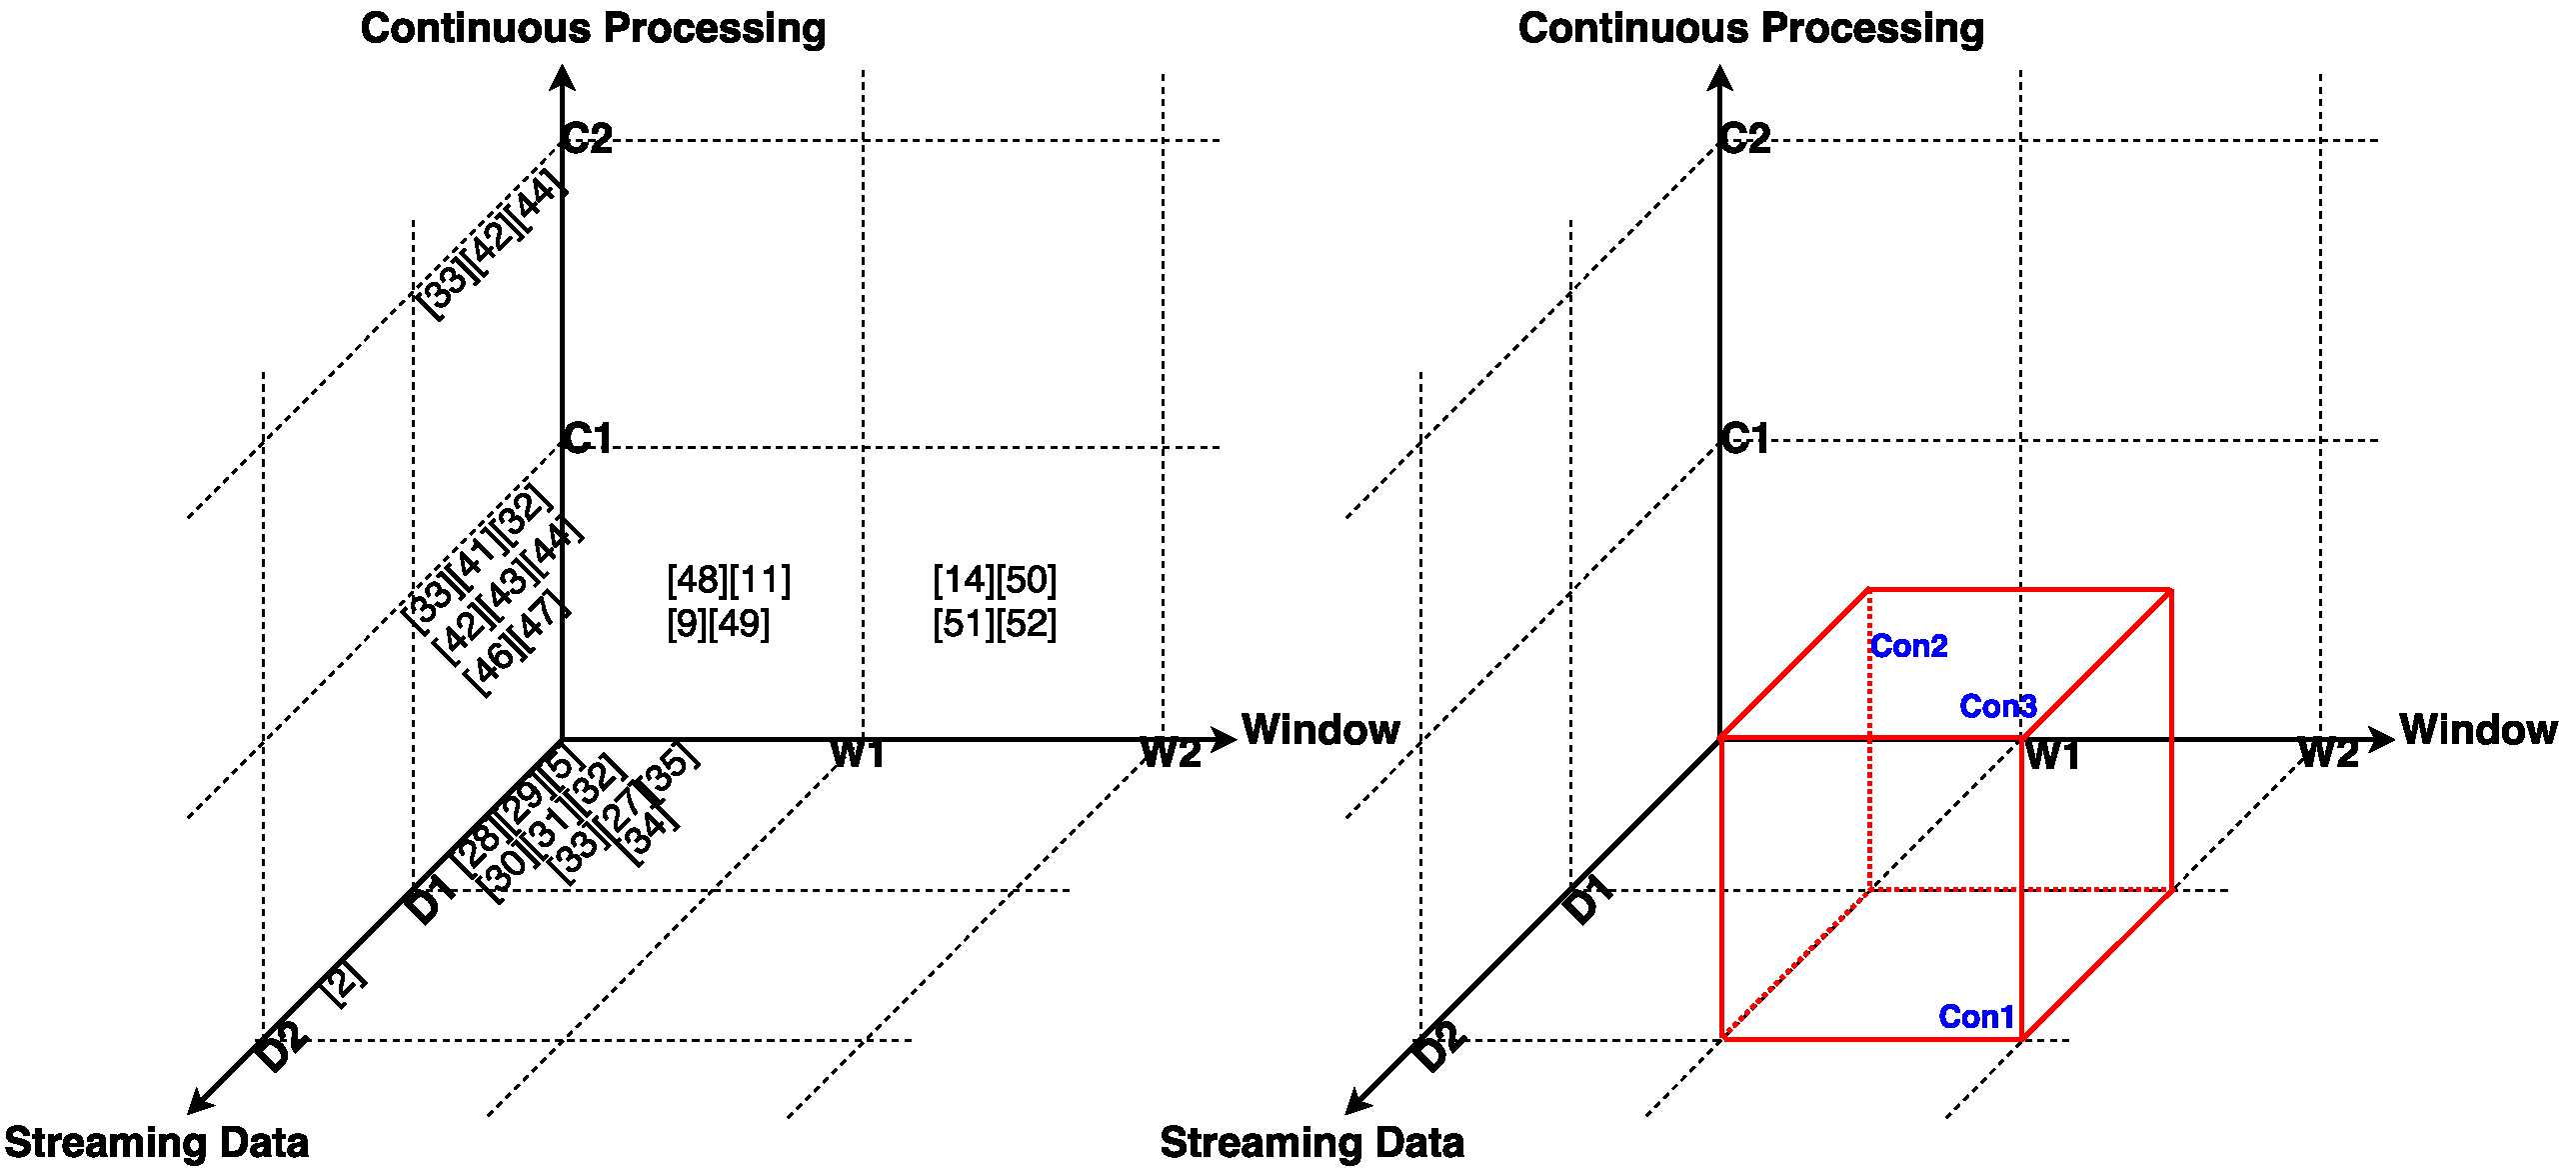
\includegraphics[width=5in]{img/2-rwc.pdf}
    \caption{Contributions in Related Work Space}
    \label{fig:2-rwc}
\end{figure}

I have plotted all the above-mentioned related work in Figure \ref{fig:2-rwc} with three dimensions of  \textbf{continuous processing}, \textbf{window} and \textbf{streaming data}.
On the continuous processing axis: 
Point C1 denotes \textit{continuous processing engine};
Point C2 denotes \textit{continuous query language}.
On the window axis:
Point W1 denotes \textit{window semantics and window operational semantics};
Point W2 denotes \textit{window management strategies}.
On the streaming data axis:
Point D1 denotes \textit{streaming data semantic modeling (RDF stream)};
Point D2 denotes \textit{streaming data orderings}.

It turns out that this figure is very helpful to illustrate and understand where the related work is. 
For example, work located in the plane of C1-D1 is about continuous processing engines that process RDF streams. 
There are some empty areas, which doesn't necessarily mean there is no work. 
The related work is definitely not an exhaust list, but are more related to this dissertation. 

Figure \ref{fig:2-rwc} also shows where my contributions can fit into this 3D space, which is the red cube. 
Contribution 1 models the data importance with the data ordering.
Contribution 2 focuses on continuous processing architecture for RDF streams, and leverages some amount of data orderings and window management strategies. 
Contribution 3 focuses on not only continuous processing for RDF streams, generalizing the semantic importance, but also enabling to take a wide range of streaming data, ontologies, queries, and window management strategies.